%% LaTeX-Beamer template for KIT design
%% by Erik Burger, Christian Hammer
%% title picture by Klaus Krogmann
%%
%% version 2.1
%%
%% mostly compatible to KIT corporate design v2.0
%% http://intranet.kit.edu/gestaltungsrichtlinien.php
%%
%% Problems, bugs and comments to
%% burger@kit.edu

\documentclass[18pt]{beamer}


%% SLIDE FORMAT

% use 'beamerthemekit' for standard 4:3 ratio
% for widescreen slides (16:9), use 'beamerthemekitwide'
\usepackage{listings}
\lstset{escapeinside={(*@}{@*)}}
\usepackage{templates/beamerthemekit}
% \usepackage{templates/beamerthemekitwide}
\usepackage{color}
\definecolor{editorGray}{rgb}{0.95, 0.95, 0.95}
\definecolor{editorOcher}{rgb}{1, 0.5, 0} % #FF7F00 -> rgb(239, 169, 0)
\definecolor{editorGreen}{rgb}{0, 0.5, 0} % #007C00 -> rgb(0, 124, 0)
\usepackage{upquote}
\lstdefinelanguage{JavaScript}{
	morekeywords={typeof, new, true, false, catch, function, return, null, catch, switch, var, if, in, while, do, else, case, break},
	morecomment=[s]{/*}{*/},
	morecomment=[l]//,
	morestring=[b]",
	morestring=[b]'
}

\lstdefinelanguage{HTML5}{
	language=html,
	sensitive=true, 
	alsoletter={<>=-},
	otherkeywords={
		% HTML tags
		<html>, <head>, <title>, </title>, <meta, />, </head>, <body>,
		<canvas, \/canvas>, <script>, </script>, </body>, </html>, <!, html>, <style>, </style>, ><
	},  
	ndkeywords={
		% General
		=,
		% HTML attributes
		charset=, id=, width=, height=,
		% CSS properties
		border:, transform:, -moz-transform:, transition-duration:, transition-property:, transition-timing-function:
	},  
	morecomment=[s]{<!--}{-->},
	tag=[s]
}

\lstset{%
	% Basic design
	backgroundcolor=\color{editorGray},
	basicstyle={\small\ttfamily},   
	frame=l,
	% Line numbers
	xleftmargin={0.75cm},
	numbers=left,
	stepnumber=1,
	firstnumber=1,
	numberfirstline=true,
	% Code design   
	keywordstyle=\color{blue}\bfseries,
	commentstyle=\color{darkgray}\ttfamily,
	ndkeywordstyle=\color{editorGreen}\bfseries,
	stringstyle=\color{editorOcher},
	% Code
	language=HTML5,
	alsolanguage=JavaScript,
	alsodigit={.:;},
	tabsize=2,
	showtabs=false,
	showspaces=false,
	showstringspaces=false,
	extendedchars=true,
	breaklines=true,        
	% Support for German umlauts
	literate=%
	{Ö}{{\"O}}1
	{Ä}{{\"A}}1
	{Ü}{{\"U}}1
	{ß}{{\ss}}1
	{ü}{{\"u}}1
	{ä}{{\"a}}1
	{ö}{{\"o}}1
}
%% TITLE PICTURE

% if a custom picture is to be used on the title page, copy it into the 'logos'
% directory, in the line below, replace 'mypicture' with the 
% filename (without extension) and uncomment the following line
% (picture proportions: 63 : 20 for standard, 169 : 40 for wide
% *.eps format if you use latex+dvips+ps2pdf, 
% *.jpg/*.png/*.pdf if you use pdflatex)

\titleimage{logologo2}

%% TITLE LOGO

% for a custom logo on the front page, copy your file into the 'logos'
% directory, insert the filename in the line below and uncomment it

%\titlelogo{mylogo}

% (*.eps format if you use latex+dvips+ps2pdf,
% *.jpg/*.png/*.pdf if you use pdflatex)

%% TikZ INTEGRATION

% use these packages for PCM symbols and UML classes
% \usepackage{templates/tikzkit}
% \usepackage{templates/tikzuml}
\usepackage{hyperref}
\usepackage[latin1]{inputenc}
\usepackage{xcolor}

% the presentation starts here

\title[HTML Basics]{HTML Basics}
%\subtitle{Something for XYZ 2009}
\author{Lena, Kristin, Charlotte}

% Bibliography

\usepackage[citestyle=authoryear,bibstyle=numeric,hyperref,backend=biber]{biblatex}
\addbibresource{templates/example.bib}
\bibhang1em

\begin{document}

% change the following line to "ngerman" for German style date and logos
\selectlanguage{ngerman}

%title page
\begin{frame}
\titlepage
\end{frame}

\section {Tagesziel}
\begin{frame}[fragile]{Tagesziel}
\begin {itemize}
\item Learning by doing!
\item Kreativ sein!
\item Deine erste eigene Webseite mit ganz vielen unterschiedlichen Elementen
\item Und wie k�nnte die zum Beispiel aussehen?
%\item Das werdet ihr am Tagesende geschafft haben: %\url{file:///C:/Users/Kristin/Documents/ungeordneter%20Unikram/web-workshop-master(3)/web-w%orkshop-master/Tag1Ergebnis/Workshop/index.html}
\end {itemize}
\end{frame}

%\section {Wochenziel}
%\begin{frame}[fragile]{Wochenziel}

%\begin{lstlisting}
%<script src="script.js"> </script>
%\end{lstlisting}

%\end{frame}

\section{Allgemeiner Aufbau}
\begin{frame}[fragile]{Was ist HTML?}
Ein Beispiel:
\begin{lstlisting}
<!DOCTYPE html>
<html>
<head>
	<title>Page Title</title>
</head>
	
<body>
	<h1>Meine erste �berschrift</h1>
	<p>Mein erster Paragraph.</p>
</body>
</html> 
\end{lstlisting}
\end{frame}

\begin{frame}[fragile]{Was ist HTML?}
\begin {itemize}
\item ausgeschrieben: Hyper Text Markup Language (deutsch: Hypertext-Auszeichnungssprache)
\item beschreibt die Struktur von Webseiten in einer maschinenlesbaren Sprache
\end {itemize}
\end{frame}

\begin{frame}[fragile]{Allgemeiner Aufbau}
\fcolorbox{red}{white}{\parbox{\linewidth}{\begin{center}Wichtig: Solange wir HTML-Code schreiben, verwenden wir Tags.\end{center}}} \\
\pause
\begin{center}Jeder Tag ist wie folgt aufgebaut:\end{center}
\begin{lstlisting}
	<tagname>Inhalt des Tags...</tagname>
\end{lstlisting}
\pause
\fcolorbox{red}{white}{\parbox{\linewidth}{\begin{center}Wichtig: Fast alle Tags, die ge\"offnet werden, m�ssen zwingend wieder geschlossen werden au�er $<$!DOCTYPE html$>$ und ein paar wenige Ausnahmen!\end{center}}}
\end{frame}

\begin{frame}[fragile]{Allgemeiner Aufbau}
\fcolorbox{red}{white}{\parbox{\linewidth}{\begin{center}Wichtig: Jeder HTML Code hat das gleiche Grundger\"ust mit grundlegenden Elementen!\end{center}}}
\end{frame}

\begin{frame}[fragile]{Allgemeiner Aufbau}
\begin{figure}
	\centering
	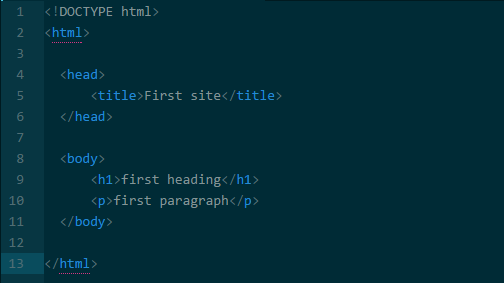
\includegraphics[width=1\textwidth]{structure2.png}
\end{figure}
\end{frame}

\begin{frame}[fragile]{Allgemeiner Aufbau}
	\textbf{Jetzt ist es endlich soweit:} \\ Erstellt eure erste eigene Website mit einem Head, einem Titel und einem Body! \\
	Erinnerung: Grundger�st
\end{frame}

\section{�berschriften}
\begin{frame}[fragile]{�berschriften und Paragraphen}
\begin{itemize}
\item F\"ur \"Uberschriften verwendet ihr die Tags $<$h1$>$ bis $<$h6$>$:
\begin{lstlisting}
	<h1>Das ist eine �berschrift</h1>
\end{lstlisting}
\pause
\item Mit $<$h1$>$ markiert ihr die wichtigste �berschrift, mit $<$h6$>$ die am wenigsten Wichtigste.
%\item Dickere \"Uberschriften k�nnt ihr erstellen in dem ihr ein den Tag wie folgt erweitert:(das Style-Attribut font-size verwendet) zu Styles verschieben
%\begin{lstlisting}
%<h1 style="font-size:60px;">�berschrift</h1>
%\end{lstlisting} 
\item Nicht sch�n? Nicht schlimm, das gestalten wir sp�ter noch!
\end{itemize}
\end{frame}

\begin{frame}[fragile]{�berschriften und Paragraphen}
\begin{itemize}
\item F�r Paragraphen verwendet ihr den Tag $<$p$>$.
\begin{lstlisting}
	<p>Das ist ein Paragraph</p>
\end{lstlisting}
\pause
\item Einen Zeilenumbruch k�nnt ihr mit $<$br$>$ herstellen.
\begin{lstlisting}
	<p>Hier entsteht ein<br>Zeilenumbruch</p>
\end{lstlisting}
\end{itemize}
\end{frame}

\begin{frame}[fragile]{�berschriften und Paragraphen}
\textbf{Eure Webseite bekommt endlich ihre ersten Elemente!} \\
F�gt eure erste �berschrift ein und schreibt direkt danach einen kleinen Paragraphen zu eurer Website.
\end{frame}

\section{Kommentare}
\begin{frame}[fragile]{Kommentare}
Um die �bersicht zu behalten, sind manchmal Kommentare sehr hilfreich!
\pause
\begin{lstlisting}
<body>
<h1>Hier steht eure �berschrift</h1>
<!-- Kommentar --> 
<p>Hier steht euer Text</p>
</body>
\end{lstlisting}
\end{frame}

\section{Styles}
\begin{frame}[fragile]{Styles}
\textbf{Jetzt wird endlich alles sch�ner!} \\
%Bedeutung Attribut + wichtig?\\
Auch der Style-Tag ist immer gleich aufgebaut:
\pause
\begin{lstlisting}
	<tagname style="eigenschaft:wert;">
\end{lstlisting}
%Verweis CSS?
\end{frame}

\begin{frame}[fragile]{Styles}
Mit dem Style-Attribut k�nnt ihr jetzt unterschiedliche Elemente kreativer gestalten. Zum Beispiel:
\begin{itemize}
\item die Hintergrundfarbe:
\begin{lstlisting}
<body style="backround-color:powderblue;">
	<h1>Das ist eine �berschrift</h1>
	<p>Das ist ein Paragraph</p>
</body>
\end{lstlisting}
\end{itemize}
\end{frame}

\begin{frame}[fragile]{Styles}
\begin{itemize}
\item die Textfarbe:
\begin{lstlisting}
<body>
	<h1 style="color:#006699;">�berschrift</h1>
	<p style="color:#006699;">Paragraph</p>
</body>	
\end{lstlisting}
\pause
\item die Schriftart:
\begin{lstlisting}
<body>
	<h1 style="font-family:verdana;">Das ist eine �berschrift</h1>
	<p> style="font-family:arial;">Das ist ein Paragraph</p>
</body>
\end{lstlisting}
\end{itemize}	
\end{frame}

\begin{frame}[fragile]{Styles}
\begin{itemize}
\item die Schriftgr��e:
\begin{lstlisting}
<body>
	<h1 style="font-size:300%;">Das ist eine �berschrift</h1>
	<p style="font-size:150%;">Das ist ein Paragraph</p>
</body>	
\end{lstlisting}
\pause
\item Positionierung des Textes: 
\begin{lstlisting}
<body>
	<h1 style="text-align:center;">Das ist eine �berschrift</h1>
	<p>Das ist ein Paragraph</p>
</body>
\end{lstlisting}
\end{itemize}
\end{frame}

\begin{frame}[fragile]{Styles}
\textbf{Endlich werden wir}
\color{orange}{k}\color{red}{r}\color{magenta}{e}\color{purple}{a}\color{yellow}{t}\color{cyan}{i}\color{green}{v}\color{black}\textbf{!} \\
Gestaltet eure Seite mit einer Hintergrund- und unterschiedlichen Textfarben und richtet Texte aus, wie es euch am besten gef�llt, aber auch sinnvoll ist.
\end{frame}

\section{Links}
\begin{frame}[fragile]{Links}
Nun binden wir Links ein, um von unserer Website zu anderen Internetseiten schnell wechseln zu k�nnen.
\pause
\\
Dazu verwenden wir:
\begin{lstlisting}
<a href="(*@\textit{url}@*)">link text</a>
\end{lstlisting}
\pause
Als Beispiel:
\begin{lstlisting}
<a href="https://www.google.com/">Google!</a>
\end{lstlisting}
\end{frame}

\begin{frame}[fragile]{Links}
\textbf{Probiert es einfach selbst!} \\
Bindet z.B. eure Facebook- oder Instagramseite ein, die Youtube-Startseite und die Zeitung Spiegel Online.
\end{frame}

\section{Bilder}
\begin{frame}[fragile]{Bilder}
Als n�chstes f�gen wir Bilder hinzu mit:
\begin{lstlisting}
<img src="(*@\textit{url}@*)">
\end{lstlisting}
\pause
Was f�llt euch auf?
\pause
\\
Als Beispiel:
\begin{lstlisting}
<img src="img-beispiel.jpg" alt="Beispielbild">
\end{lstlisting}
\end{frame}

\begin{frame}[fragile]{Bilder}
\begin{center}
\textbf{Endlich k�nnen wir s��e Tierbilder \\ einf�gen!}
\begin{figure}
	\centering
	
\includegraphics[width=0.4\textwidth]{igel.jpg}
\end{figure}
Und genau das machen wir jetzt auch: Sucht euch ein Bild oder mehrere mit einem Motiv eurer Wahl und f�gt sie in eure Website unter euren Paragraphen ein.
\end{center}
\end{frame}

\section{Iframes}
\begin{frame}[fragile]{Iframes}
\begin{itemize}
\item Iframes werden benutzt, um eine Webseite in einer Webseite darzustellen
\item WAS?! Das ganze mal anschaulich! %Direkt zeigen im Code und wie es schlussendlich aussieht
\end{itemize}
\end{frame}

\begin{frame}[fragile]{Iframes}
\textbf{Wann braucht man so etwas?} \\
Iframes ben�tigen wir beispielsweise beim Einbinden von Gifs:
\begin{lstlisting}
<iframe src="(*@\textit{url}@*)"> </iframe>
\end{lstlisting}
\pause
H�he und Breite legen wir so fest:
\begin{lstlisting}
<iframe src="(*@\textit{url}@*)" height="200" width="300"> </iframe>
\end{lstlisting}
\end{frame}

\begin{frame}[fragile]{Iframes}
Das ist aber noch nicht alles, was man mit Iframes machen kann.\\
Auch Videos bindet ihr damit ganz leicht ein:
\begin{lstlisting}
<iframe src="(*@\textit{url}@*)" height="200" weight="300"><\iframe>
\end{lstlisting}
Was f�llt euch auf?
\pause
Mit der Erg�nzung \textit{allowfullscreen} k�nnt ihr dem Nutzer das Video sogar im Vollbildmodus zeigen.
\end{frame}

\begin{frame}[fragile]{Iframes}
\textbf{Dann legt mal los:} \\
Sucht euch auf giphy.com ein cooles Gif aus und f�gt es �ber oder unter eurem Bild ein. \\
Die Umrandung ist nicht sch�n? Kein Problem, ein kleiner Trick:
\begin{lstlisting}
<iframe src="(*@\textit{url}@*)" height="200" width="300" frameBorder="0"> </iframe>
\end{lstlisting}
Und jetzt fehlt uns nur noch ein Youtube-Video! Bindet also auch das einfach mit dem Iframe-Tag ein.
\end{frame}

\section{Listen}
\begin{frame}[fragile]{Listen}
Zu allerletzt fehlen uns nur noch Listen:
\pause
\begin{lstlisting}
<p>
	<ul>
		<li>Nummer 1</li>
		<li>Nummer 2</li>
		<li>Nummer 3</li>
	</ul>
</p>	
\end{lstlisting}
\end{frame}

\begin{frame}[fragile]{Listen}
Erstellt eine Liste 
\begin{itemize}
\item von euren Hobbys,
\item von Dingen, die ihr gern macht oder
\item von Dingen, die ihr irgendwann mal machen m�chtet!
\end{itemize}
\end{frame}

\end{document}
